\section{Operaciones básicas}
\begin{enumerate}
% Basic
    \item \textbf{Doble}\\
    Escribe un programa que lea de la consola un número entero y muestre en la consola su doble.
    \subsection*{Ejemplos:}
    \begin{itemize}
        \item Entrada: \texttt{4}\\
              Salida: \texttt{8}
        \item Entrada: \texttt{-5}\\
              Salida: \texttt{-10}
        \item Entrada: \texttt{0}\\
              Salida: \texttt{0}
    \end{itemize}
    
    \item \textbf{Área de un triángulo}\\
    Escribe un programa que lea de la consola la base \(b\) y la altura \(h\) de un triángulo, calcule su área y la escriba en la consola.\\
    \[
    \text{Área} = \frac{b \cdot h}{2}
    \]
    \subsection*{Ejemplos:}
    \begin{itemize}
        \item Entrada: \texttt{b = 10, h = 5}\\
              Salida: \texttt{Área = 25}
        \item Entrada: \texttt{b = 3, h = 4}\\
              Salida: \texttt{Área = 6}
    \end{itemize}

    \item \textbf{Promedio de tres números}\\
    Escribe un programa que lea tres números reales \(x\), \(y\) y \(z\) de la consola, calcule su promedio y lo muestre en la consola.
    \subsection*{Ejemplos:}
    \begin{itemize}
        \item Entrada: \texttt{3.0, 4.0, 5.0}\\
              Salida: \texttt{Promedio = 4.0}
        \item Entrada: \texttt{-1.0, -2.0, -3.0}\\
              Salida: \texttt{Promedio = -2.0}
        \item Entrada: \texttt{10.5, 20.5, 30.5}\\
              Salida: \texttt{Promedio = 20.5}
    \end{itemize}

    \item \textbf{Cambio de temperatura}\\
    Escribe un programa que lea de la consola una temperatura en grados Fahrenheit (\(F\)), la convierta a grados Celsius (\(C\)) y muestre el resultado en la consola.\\ 
    \[
    C = \frac{5}{9} \cdot (F - 32)
    \]
    \subsection*{Ejemplos:}
    \begin{itemize}
        \item Entrada: \texttt{F = 50}\\
              Salida: \texttt{C = 10}
        \item Entrada: \texttt{F = 32}\\
              Salida: \texttt{C = 0}
        \item Entrada: \texttt{F = 100}\\
              Salida: \texttt{C = 37.78}
    \end{itemize}

    \item \textbf{Perímetro y área de un círculo}\\
    Escribe un programa que lea de la consola el radio \(r\) de un círculo, calcule su perímetro y su área, y muestre ambos resultados en la consola.\\   
    \[
    \text{Perímetro} = 2\pi r, \quad \text{Área} = \pi r^2
    \]
    \subsection*{Ejemplos:}
    \begin{itemize}
        \item Entrada: \texttt{r = 3}\\
              Salida: \texttt{Perímetro = 18.8496, Área = 28.2744}
        \item Entrada: \texttt{r = 0}\\
              Salida: \texttt{Perímetro = 0, Área = 0}
        \item Entrada: \texttt{r = 1.5}\\
              Salida: \texttt{Perímetro = 9.4248, Área = 7.0686}
    \end{itemize}

    \item \textbf{Hipotenusa}\\
    Escribe un programa que lea de la consola los catetos \(a\) y \(b\) de un triángulo rectángulo, calcule la longitud de su hipotenusa y la escriba en la consola.\\
    \[
    c = \sqrt{a^2 + b^2}
    \]
    \subsection*{Ejemplos:}
    \begin{itemize}
        \item Entrada: \texttt{a = 3, b = 4}\\
              Salida: \texttt{c = 5}
        \item Entrada: \texttt{a = 5, b = 12}\\
              Salida: \texttt{c = 13}
        \item Entrada: \texttt{a = 8, b = 15}\\
              Salida: \texttt{c = 17}
    \end{itemize}

% Intermediate
    \item \textbf{Suma de dígitos}\\
    Escribe un programa que lea un número entero de tres cifras \(n\) de la consola, calcule la suma de sus dígitos y la muestre en la consola.\\
    Ejemplo: Si \(n = 123\), entonces:
    \[
    \text{suma} = 1 + 2 + 3
    \]
    Pista: Usa la división y resto de la división para extraer los dígitos:
    \[
    \text{Centena} = \frac{n}{100}, \quad \text{Decena} = \frac{(n \% 100)}{10}, \quad \text{Unidad} = n \% 10
    \]
    \subsection*{Ejemplos:}
    \begin{itemize}
        \item Entrada: \texttt{n = 123}\\
              Salida: \texttt{Suma = 6}
        \item Entrada: \texttt{n = 456}\\
              Salida: \texttt{Suma = 15}
        \item Entrada: \texttt{n = 789}\\
              Salida: \texttt{Suma = 24}
    \end{itemize}
    
    \item \textbf{Distancia entre dos puntos}\\
    Escribe un programa que lea de la consola las coordenadas de dos puntos \( (x_1, y_1) \) y \( (x_2, y_2) \) en el plano, calcule la distancia entre ellos y escriba el resultado en la consola.\\
    \[
    \text{Distancia} = \sqrt{(x_2 - x_1)^2 + (y_2 - y_1)^2}
    \]
    \subsection*{Ejemplos:}
    \begin{itemize}
        \item Entrada: \texttt{(x1 = 1, y1 = 2), (x2 = 4, y2 = 6)}\\
              Salida: \texttt{Distancia = 5}
        \item Entrada: \texttt{(x1 = 0, y1 = 0), (x2 = 3, y2 = 4)}\\
              Salida: \texttt{Distancia = 5}
        \item Entrada: \texttt{(x1 = -1, y1 = -1), (x2 = 2, y2 = 3)}\\
              Salida: \texttt{Distancia = 5}
    \end{itemize}

    \item \textbf{Ecuación cuadrática}\\
    Reciba los coeficientes \(a\), \(b\) y \(c\) (números reales) de una ecuación cuadrática de la forma:

\[
ax^2 + bx + c = 0
\]

y, asumiendo que la ecuación tiene dos soluciones reales, calcule las raíces de la ecuación utilizando la fórmula cuadrática:

\[
x = \frac{-b \pm \sqrt{b^2 - 4ac}}{2a}
\]

Se asegura que el discriminante (\(\Delta = b^2 - 4ac\)) es mayor que 0 para que existan dos soluciones reales.

\subsection*{Ejemplos}
\begin{itemize}
    \item Entrada: \texttt{a = 1, b = -3, c = 2}\\
          Salida: \texttt{x1 = 2, x2 = 1}
    \item Entrada: \texttt{a = 2, b = 5, c = -3}\\
          Salida: \texttt{x1 = 0.5, x2 = -3}
    \item Entrada: \texttt{a = 1, b = -6, c = 8}\\
          Salida: \texttt{x1 = 4, x2 = 2}
\end{itemize}


\subsection*{Más avanzados}
% Advanced
    \item \textbf{Minutos a horas}\\
    Escribe un programa que lea un número entero \(t\) que representa una cantidad de minutos de la consola, calcule cuántas horas completas y cuántos minutos sobran, y muestre ambos valores en la consola.\\
    \textbf{Pista:} Usa la división y resto de la división para manejar cuando te pases de 60:
    \[
    \text{Horas} = \frac{t}{60}, \quad \text{Minutos} = t \% 60
    \]
    \subsection*{Ejemplos:}
    \begin{itemize}
    \item Entrada: \texttt{t = 130}\\
          Salida: \texttt{Horas = 2, Minutos = 10}
    \item Entrada: \texttt{t = 75}\\
          Salida: \texttt{Horas = 1, Minutos = 15}
    \item Entrada: \texttt{t = 45}\\
          Salida: \texttt{Horas = 0, Minutos = 45}
\end{itemize}
    
    \item \textbf{Mayor}\\
    Reciba dos números enteros de la consola y determine cuál de los dos es mayor sin utilizar $Math.Max$ y $Math.Min$. No utilice condicionales.
    \subsection*{Ejemplos:}
    \begin{itemize}
    \item Entrada: \texttt{a = 5, b = 10}\\
          Salida: \texttt{Mayor = 10}
    \item Entrada: \texttt{a = -3, b = -7}\\
          Salida: \texttt{Mayor = -3}
    \item Entrada: \texttt{a = 12, b = 12}\\
          Salida: \texttt{Mayor = 12}
    \end{itemize}
    
    \item \textbf{Valor medio}\\
    Reciba tres números enteros. Muestre en la consola el de valor medio (Utilice $Math.Max$ y $Math.Min$) y el promedio de estos.
    \begin{itemize}
    \subsection*{Ejemplos:}
    \item Entrada: \texttt{a = 5, b = 10, c = 15}\\
          Salida: \texttt{Valor medio = 10, Promedio = 10}
    \item Entrada: \texttt{a = -3, b = 4, c = 8}\\
          Salida: \texttt{Valor medio = 4, Promedio = 3}
    \item Entrada: \texttt{a = 7, b = 7, c = 7}\\
          Salida: \texttt{Valor medio = 7, Promedio = 7}
\end{itemize}
        
    \item \textbf{Intercambio de variables}\\
    Dado que tienes dos enteros guardados en las variables \(a\) y \(b\), realiza el intercambio de sus valores de las siguientes maneras:

\begin{enumerate}
    \item Usando una variable auxiliar.
    \item Sin usar una variable auxiliar.
\end{enumerate}

\subsection*{Ejemplo:} 
Supongamos que las variables inicializan de la siguiente manera:
\begin{lstlisting}
    int a = 5;
    int b = 9;
\end{lstlisting}

si al final de tu programa  añades la línea:
\begin{lstlisting}
    Console.WriteLine($"El valor de a es {a} y el valor de b es {b}.");
\end{lstlisting}

La salida esperada en la consola es:
\begin{verbatim}
    El valor de a es 9 y el valor de b es 5.
\end{verbatim}


    \item \textbf{Circunferencias}\\
    Sean las circunferencias $C_1$ y $C_2$ de redio $r$. Lea de la consola el radio $r$ (puede ser cualquier número real, no solo entero) y calcule el área sombreada.

\begin{center}
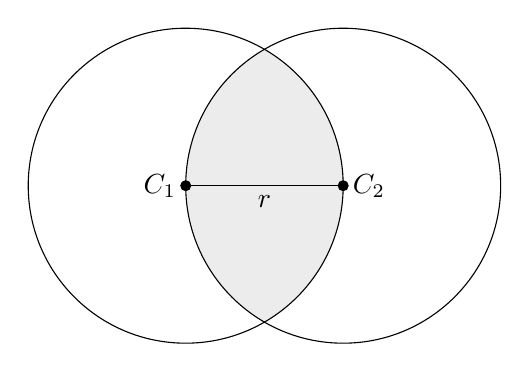
\begin{tikzpicture}
    % Definir el radio
    \def\r{2}

    % Sombrear el área de intersección
    \begin{scope}
        \clip (0,0) circle (\r);
        \fill[gray!15] (\r,0) circle (\r);
    \end{scope}

    % Dibujar la primera circunferencia
    \draw (0,0) circle (\r);

    % Dibujar la segunda circunferencia con un radio coincidente
    \draw (\r,0) circle (\r);

    % Marcar los centros de las circunferencias
    \fill (0,0) circle (2pt) node[left] {$C_1$};
    \fill (\r,0) circle (2pt) node[right] {$C_2$};

    % Dibujar el radio coincidente y etiquetarlo
    \draw (0,0) -- (\r,0) node[midway, below] {$r$};
\end{tikzpicture}
\end{center}

\subsection*{Ejemplos}
\begin{itemize}
    \item Entrada: \texttt{3}\\
          Salida: \texttt{El área sombreada es: 18.84955592153876}
    \item Entrada: \texttt{5}\\
          Salida: \texttt{El área sombreada es: 52.35987755982988}
    \item Entrada: \texttt{10}\\
          Salida: \texttt{El área sombreada es: 209.43951023931953}
\end{itemize}


    \item \textbf{Velocidad de escritura}\\
    Lea un texto de la terminal y muestre en la consola la velocidad de escritura del usuario que ingresó dicho texto.

Investigue cómo utilizar Environment.TickCount para medir la cantidad de milisegundos transcurridos.

    \item \textbf{Fecha de nacimiento}\\
    Reciba de la consola el número de identidad de una persona como tipo \textit{long} e imprima su fecha de nacimiento con el formato  \texttt{día/mes/año}.

El año puede mostrarse con las dos cifras presentes en el carnet, por ejemplo, para el carnet \texttt{04100968518}, la fecha de nacimiento sería \texttt{9/10/4}.

\subsection*{Ejemplos:}
\begin{itemize}
    \item Entrada: \texttt{04100968518}\\
          Salida: \texttt{9/10/4}
    \item Entrada: \texttt{15020358645}\\
          Salida: \texttt{3/2/15}
    \item Entrada: \texttt{31071254567}\\
          Salida: \texttt{12/7/31}
\end{itemize}
\end{enumerate}

\newpage
\section{Condicionales}
\begin{enumerate}
% Basic 
    \item \textbf{Número positivo, negativo o cero}\\
    Escribe un programa que lea un número entero y determine si es positivo, negativo o igual a cero.
    \subsection*{Ejemplos:}
    \begin{itemize}
        \item Entrada: \texttt{-5}\\
              Salida: \texttt{El número es negativo.}
        \item Entrada: \texttt{0}\\
              Salida: \texttt{El número es igual a cero.}
        \item Entrada: \texttt{8}\\
              Salida: \texttt{El número es positivo.}
    \end{itemize}

    \item \textbf{Mayor de dos números}\\
    Lee dos números enteros y muestra cuál de ellos es mayor, o indica si son iguales.
    \subsection*{Ejemplos:}
    \begin{itemize}
        \item Entrada: \texttt{12, 7}\\
              Salida: \texttt{El número mayor es 12.}
        \item Entrada: \texttt{4, 9}\\
              Salida: \texttt{El número mayor es 9.}
        \item Entrada: \texttt{10, 10}\\
              Salida: \texttt{Ambos números son iguales.}
    \end{itemize}

    \item \textbf{Par o impar}\\
    Escribe un programa que determine si un número entero no negativo dado es par o impar.
    \subsection*{Ejemplos:}
    \begin{itemize}
        \item Entrada: \texttt{6}\\
              Salida: \texttt{El número es par.}
        \item Entrada: \texttt{13}\\
              Salida: \texttt{El número es impar.}
        \item Entrada: \texttt{0}\\
              Salida: \texttt{El número es par.}
    \end{itemize}

    \item \textbf{Calificación}\\
    Lee una calificación numérica (de 0 a 100) y determina si el estudiante aprobó o reprobó (se aprueba con 60 o más).
    \subsection*{Ejemplos:}
    \begin{itemize}
        \item Entrada: \texttt{75}\\
              Salida: \texttt{El estudiante aprobó.}
        \item Entrada: \texttt{50}\\
              Salida: \texttt{El estudiante reprobó.}
        \item Entrada: \texttt{60}\\
              Salida: \texttt{El estudiante aprobó.}
    \end{itemize}
    
    \item \textbf{Divisible}\\
    Implemente un programa que reciba dos enteros y determine si el primero es divisible por el segundo.
\subsection*{Ejemplos:}
\begin{itemize}
    \item Entrada: \texttt{10, 2}\\
          Salida: \texttt{10 es divisible por 2.}
    \item Entrada: \texttt{15, 4}\\
          Salida: \texttt{15 no es divisible por 4.}
    \item Entrada: \texttt{20, 5}\\
          Salida: \texttt{20 es divisible por 5.}
    \item Entrada: \texttt{7, 3}\\
          Salida: \texttt{7 no es divisible por 3.}
\end{itemize}


    \item \textbf{Valor absoluto}\\
    Implemente un programa que reciba un número entero \( x \) de la consola y calcule su valor absoluto. El valor absoluto de un número \( x \) se define como el número sin su signo, es decir, la distancia de \( x \) al origen en la recta numérica. No utilice Math.Abs.

La función del valor absoluto \( |x| \) se define de la siguiente manera:
\[
|x| =
\begin{cases} 
x & \text{si } x \geq 0 \\
-x & \text{si } x < 0
\end{cases}
\]

\subsection*{Ejemplos}
\begin{itemize}
    \item Entrada: 5
    
    Salida: El valor absoluto de 5 es: 5

    \item Entrada: -8
    
    Salida: El valor absoluto de -8 es: 8

    \item Entrada: 0
    
    Salida: El valor absoluto de 0 es: 0
\end{itemize}


% Intermediate
    \item \textbf{Mayor de 3}\\
    Implemente un programa que lea tres enteros de la consola e imprima el mayor.
\subsection*{Ejemplos:}
\begin{itemize}
    \item Entrada: \texttt{3, 5, 2}\\
          Salida: \texttt{El mayor número es 5.}
    \item Entrada: \texttt{10, 7, 10}\\
          Salida: \texttt{El mayor número es 10.}
    \item Entrada: \texttt{-1, -5, -3}\\
          Salida: \texttt{El mayor número es -1.}
    \item Entrada: \texttt{8, 8, 8}\\
          Salida: \texttt{El mayor número es 8.}
\end{itemize}

    \item \textbf{Categoría de edad}\\
    Escribe un programa que clasifique a una persona según su edad:
    \begin{itemize}
        \item Niño (0-12 años)
        \item Adolescente (13-17 años)
        \item Adulto (18-64 años)
        \item Adulto mayor (65 o más años)
    \end{itemize}
    \subsection*{Ejemplos:}
    \begin{itemize}
        \item Entrada: \texttt{7}\\
              Salida: \texttt{Niño}
        \item Entrada: \texttt{15}\\
              Salida: \texttt{Adolescente}
        \item Entrada: \texttt{30}\\
              Salida: \texttt{Adulto}
        \item Entrada: \texttt{65}\\
              Salida: \texttt{Adulto mayor}
    \end{itemize}

    \item \textbf{Triángulo válido}\\
    Dados tres números que representan las longitudes de los lados de un triángulo, determina si forman un triángulo válido. Un triángulo es válido si la suma de las longitudes de dos lados es mayor que la longitud del tercer lado para cualquier combinación de lados.
    \subsection*{Ejemplos:}
    \begin{itemize}
        \item Entrada: \texttt{3, 4, 5}\\
              Salida: \texttt{Triángulo válido}
        \item Entrada: \texttt{1, 2, 3}\\
              Salida: \texttt{No es un triángulo válido}
        \item Entrada: \texttt{6, 8, 10}\\
              Salida: \texttt{Triángulo válido}
    \end{itemize}

    \item \textbf{Número dentro de un rango}\\
    Lee tres números \(a\), \(b\), y \(x\) (donde \(a \leq b\)) y determina si \(x\) se encuentra dentro del rango cerrado \([a, b]\).
    \subsection*{Ejemplos:}
    \begin{itemize}
        \item Entrada: \texttt{2, 8, 5}\\
              Salida: \texttt{Sí, 5 está dentro del rango [2, 8].}
        \item Entrada: \texttt{1, 10, 15}\\
              Salida: \texttt{No, 15 no está dentro del rango [1, 10].}
        \item Entrada: \texttt{3, 9, 9}\\
              Salida: \texttt{Sí, 9 está dentro del rango [3, 9].}
    \end{itemize}

% Advanced
    \item \textbf{Días en un mes}\\
    Escribe un programa que lea un número que representa un mes (1 para enero, 2 para febrero, etc.) y muestre la cantidad de días que tiene ese mes. Considera años no bisiestos, o sea, febrero siempre tendría 28 días.
    \subsection*{Ejemplos:}
    \begin{itemize}
        \item Entrada: \texttt{1}\\
              Salida: \texttt{31 días}
        \item Entrada: \texttt{2}\\
              Salida: \texttt{28 días}
        \item Entrada: \texttt{4}\\
              Salida: \texttt{30 días}
    \end{itemize}

    \item \textbf{Año bisiesto}\\
    Escribe un programa que determine si un año es bisiesto o no. Un año es bisiesto si es divisible entre 4, pero no es divisible entre 100, a menos que también sea divisible entre 400.
    \subsection*{Ejemplos:}
    \begin{itemize}
        \item Entrada: \texttt{2020}\\
              Salida: \texttt{El año 2020 es bisiesto.}
        \item Entrada: \texttt{1900}\\
              Salida: \texttt{El año 1900 no es bisiesto.}
        \item Entrada: \texttt{2000}\\
              Salida: \texttt{El año 2000 es bisiesto.}
    \end{itemize}

    \item \textbf{Calculadora básica}\\
    Implemente un programa que lea de la consola dos enteros y un operador (+, -, /, *) y realice la operación correspondiente entre ellos e imprima el resultado en consola.
\begin{itemize}
    \item Entrada: \texttt{5, 3, +}\\
    Salida: \texttt{El resultado de 5 + 3 es: 8}
    
    \item Entrada: \texttt{10, 4, -}\\
    Salida: \texttt{El resultado de 10 - 4 es: 6}
    
    \item Entrada: \texttt{8, 7, *}\\
    Salida: \texttt{El resultado de 8 * 7 es: 56}
    
    \item Entrada: \texttt{9, 3, /}\\
    Salida: \texttt{El resultado de 9 / 3 es: 3}
    
    \item Entrada: \texttt{5, 0, /}\\
    Salida: \texttt{Error: División por cero.}
\end{itemize}

\subsection*{Más avanzados}
    \item \textbf{Cálculo de tarifas}\\
    Escribe un programa que calcule el costo de estacionamiento según el tiempo de permanencia:
    \begin{itemize}
        \item Primera hora: \$70
        \item Horas adicionales: \$50 cada una
        \item Máximo diario: \$1000
    \end{itemize}
    Lee el tiempo de permanencia (en horas) y calcula el costo total.
    \subsection*{Ejemplos:}
    \begin{itemize}
        \item Entrada: \texttt{1}\\
              Salida: \texttt{El costo total es: \$70}
        \item Entrada: \texttt{5}\\
              Salida: \texttt{El costo total es: \$270}
        \item Entrada: \texttt{20}\\
              Salida: \texttt{El costo total es: \$1000}
    \end{itemize}
    
    \item \textbf{Determinando el sexo}\\
    Implemente un programa que le pida al usuario su número de identidad y determine su sexo. El sexo puede determinarse por el penúltimo dígito del número de identidad (par masculino, impar femenino).

\subsection*{Ejemplos}
\begin{itemize}
    \item Entrada: \texttt{02020966175}\\
          Salida: \texttt{Femenino}
    
    \item Entrada: \texttt{04102566345}\\
          Salida: \texttt{Masculino}
    
    \item Entrada: \texttt{05031278457}\\
          Salida: \texttt{Femenino}
\end{itemize}


\end{enumerate}

\newpage
\section{Métodos}
\begin{enumerate}
% Basic
    \item \textbf{Validando horas}\\
     Dada una hora en formato de 24 horas representada por dos enteros horas y minutos, determine si es válida o no.
     \subsection*{Ejemplos:}
    \begin{itemize}
        \item Entrada: \texttt{h = 13, m = 45}\\
              Salida: \texttt{La hora es válida.}
        \item Entrada: \texttt{h = 25, m = 10}\\
              Salida: \texttt{La hora no es válida.}
        \item Entrada: \texttt{h = 7, m = 60}\\
              Salida: \texttt{La hora no es válida.}
        \item Entrada: \texttt{h = 0, m = 0}\\
              Salida: \texttt{La hora es válida.}
        \item Entrada: \texttt{h = 23, m = 59}\\
              Salida: \texttt{La hora es válida.}
    \end{itemize}

     \item \textbf{Tipo de triángulo}\\
    Implemente un programa que pida al usuario tres números enteros qque representen los lados de un triángulo y determine qué tipo de triángulo forman. Debe mostrar en la consola lo siguiente:
\begin{itemize}
	\item 0 si no pueden ser lados de ningún triángulo
	\item 1 si es un triángulo escaleno
	\item 2 si es un triángulo isóceles
	\item 3 si es un triángulo equilátero
\end{itemize}

\textbf{Propuesta:} Realizar la implementación utilizando \textcolor{blue}{enum}.

\subsection*{Ejemplos}
\begin{itemize}
    \item Entrada: side1 = 1, side2 = 2, side3 = 3

    Salida: 0

    \item Entrada: side1 = 3, side2 = 4, side3 = 5

    Salida: 1

    \item Entrada: side1 = 4, side2 = 4, side3 = 5

     Salida: 2

     \item Entrada: side1 = 6, side2 = 6, side3 = 6
     
     Salida: 3
\end{itemize}


% Intermediate
    \item \textbf{Validando fechas}\\
    Lea tres números enteros de la consola que representarán día, mes y año respectivamente. Si estos valores pueden formar una fecha, entonces muéstrela en la consola con el formato \texttt{día/mes/año}, si no imprima el No es fecha. Considere que las fechas con año menor que 1 no son válidas.

\subsection*{Ejemplos}
\begin{itemize}
    \item Entrada: d = 15, m = 8, y = 0\\
    Salida: No es fecha\\
    Explicación: El año 0 no es válido

    \item Entrada: d = 15, m = 13, y = 2023\\
    Salida: No es fecha\\
    Explicación: El mes 13 no es válido
    
    \item Entrada: d = 31, m = 4, y = 2023\\
    Salida: No es fecha\\
    Explicación: Abril tiene solo 30 días

    \item Entrada: d = 15, m = 8, y = 2023\\
    Salida: 15/8/2023
    
    \item Entrada: d = 29, m = 2, y = 2020\\
    Salida: 29/2/2020\\
    Explicación: 2020 es un año bisiesto

    \item Entrada: d = 29, m = 2, y = 2023\\
    Salida: No es fecha\\
    Explicación: 2023 no es un año bisiesto
    
\end{itemize}
    
    \item \textbf{Conversión de Hora} \\
    Escribe un método que reciba una hora en formato de 24 horas representada por dos enteros horas y minutos y devuelva una cadena que represente la hora en formato de 12 horas, incluyendo ``AM'' o ``PM''.
    \subsection*{Ejemplos}
    \begin{itemize}
        \item Entrada: h = 14, m = 30 (\texttt{"14:30"})\\
              Salida: \texttt{"2:30 PM"}
        \item Entrada: h - 9, m = 15 (\texttt{"09:15"})\\
              Salida: \texttt{"9:15 AM"}
        \item Entrada: h = 0, m = 0 (\texttt{"00:00"})\\
              Salida: \texttt{"12:00 AM"}
        \item Entrada: h = 12, m = 12 (\texttt{"12:00"})\\
              Salida: \texttt{"12:00 M"}
    \end{itemize}

\subsection*{Más avanzados}
    % \item \textbf{Factorial}\\
    % El factorial de un número $n$ (denotado como $n!$) se define como el producto de todos los números enteros positivos desde 1 hasta $n$, o sea:

\[
n! = \prod_{k=1}^{n} k
\]

o lo que es lo mismo:

\[
n! =
\begin{cases} 
1 & \text{si } n = 0 \\
n \cdot (n-1)! & \text{si } n > 0
\end{cases}
\]

Implemente un programa que reciba un número entero no negativo \(n\) de la consola y calcule el factorial de ese número.

\subsection*{Ejemplos:}
\begin{itemize}
    \item Entrada: \texttt{0}\\
          Salida: \texttt{El factorial de 0 es 1.}
    \item Entrada: \texttt{1}\\
          Salida: \texttt{El factorial de 1 es 1.}
    \item Entrada: \texttt{5}\\
          Salida: \texttt{El factorial de 5 es 120.}
    \item Entrada: \texttt{7}\\
          Salida: \texttt{El factorial de 7 es 5040.}
\end{itemize}

    % No utilice ciclos.

    % \item \textbf{Imprimiendo números}
    % \begin{enumerate}[label=\alph*)]
    \item Implemente un método que reciba un entero $n$ y muestre en la consola en orden descendente, todos los números enteros entre $n$ y 0. No utilice ciclos.
    \item Implemente un método que reciba un entero $n$ y muestre en la consola, en orden ascendente, todos los números enteros entre 0 y $n$. No utilice ciclos.
\end{enumerate}

    \item \textbf{Día siguiente}\\
    Implemente un programa que reciba una fecha e imprima la fecha correspondiente al d siguiente.

\subsection*{Ejemplos}
\begin{itemize}
    \item Entrada: d = 10, m = 3, y = 2024

    Salida: La fecha siguiente es: 11/3/2024

    \item Entrada: d = 28, m = 2, y = 2024

    Salida: La fecha siguiente es: 29/2/2024

    \item Entrada: d = 31, m = 12, y = 2024

    Salida: La fecha siguiente es: 01/1/2025

    \item Entrada: d = 30, m = 4, y = 2024

    Salida: La fecha siguiente es: 01/5/2025
\end{itemize}


    \item \textbf{Horas}
    \begin{enumerate}[label=\alph*)]
    \item Escriba un programa que, dada una hora inicial en formato de 24 horas (representada por dos enteros: horas y minutos) y un intervalo de tiempo (también representado por dos enteros: horas y minutos), calcule la nueva hora tras sumar el intervalo al tiempo inicial. Asegúrese de ajustar los minutos y las horas para mantener el formato de 24 horas.
    \subsection*{Ejemplos}
    \begin{itemize}
        \item Entrada: \(h = 3, m = 30, \Delta h = 0, \Delta m = 70\)\\
              Salida: \texttt{La nueva hora es 4:40.}
        \item Entrada: \(h = 10, m = 45, \Delta h = 1, \Delta m = 30\)\\
              Salida: \texttt{La nueva hora es 12:15.}
        \item Entrada: \(h = 23, m = 50, \Delta h = 2, \Delta m = 20\)\\
              Salida: \texttt{La nueva hora es 2:10.}
        \item Entrada: \(h = 6, m = 10, \Delta h = 0, \Delta m = 50\)\\
              Salida: \texttt{La nueva hora es 7:00.}
        \item Entrada: \(h = 14, m = 30, \Delta h = 9, \Delta m = 90\)\\
              Salida: \texttt{La nueva hora es 0:00.}
    \end{itemize}

    \item Escriba un programa que, dada la hora de salida de un avión y su hora de llegada (ambas representadas por dos enteros: horas y minutos en formato de 24 horas), determine el tiempo total de vuelo. Asegúrese de manejar correctamente los casos en los que el vuelo cruza la medianoche.\\
    Se asegura que:
    \begin{itemize}
        \item El tiempo de vuelo no excederá las \(24\) horas.
        \item No hay cambios de zonas horarias.
    \end{itemize}
    % \textbf{Pista:} Convierta las horas y minutos a un único valor en minutos, calcule la diferencia y convierta el resultado de vuelta a horas y minutos.
    \subsection*{Ejemplos}
    \begin{itemize}
        \item Entrada: \(h_{\text{salida}} = 10, m_{\text{salida}} = 20, h_{\text{llegada}} = 13, m_{\text{llegada}} = 50\)\\
              Salida: \texttt{El tiempo de vuelo es 3 horas y 30 minutos.}
        \item Entrada: \(h_{\text{salida}} = 23, m_{\text{salida}} = 45, h_{\text{llegada}} = 2, m_{\text{llegada}} = 15\)\\
              Salida: \texttt{El tiempo de vuelo es 2 horas y 30 minutos.}
        \item Entrada: \(h_{\text{salida}} = 14, m_{\text{salida}} = 0, h_{\text{llegada}} = 14, m_{\text{llegada}} = 0\)\\
              Salida: \texttt{El tiempo de vuelo es 0 horas y 0 minutos.}
        \item Entrada: \(h_{\text{salida}} = 5, m_{\text{salida}} = 30, h_{\text{llegada}} = 8, m_{\text{llegada}} = 10\)\\
              Salida: \texttt{El tiempo de vuelo es 2 horas y 40 minutos.}
    \end{itemize}
\end{enumerate}


    \item \textbf{Signo zodiacal}\\
    Implemente un método que dado el carnet de identidad de una persona devuelva su signo del zodiaco.

\textbf{Propuesta:} Realizar la implementación utilizando \textcolor{blue}{enum}.

\subsection*{Ejemplos:}
\begin{itemize}
    \item Entrada: \texttt{02042366175} (23 de abril)\\
          Salida: \texttt{Tauro}
    \item Entrada: \texttt{02031566175} (15 de marzo)\\
          Salida: \texttt{Piscis}
    \item Entrada: \texttt{02121966175} (19 de diciembre)\\
          Salida: \texttt{Sagitario}
    \item Entrada: \texttt{03110178934} (1 de noviembre)\\
          Salida: \texttt{Escorpio}
    \item Entrada: \texttt{05123078934} (30 de diciembre)\\
          Salida: \texttt{Capricornio}
\end{itemize}



% Advanced
    \item \textbf{Día de la semana}\\
    Implemente un programa que dada una fecha, muestre qué day de la semana cae.

\textbf{Propuesta:} Realizar la implementación utilizando \textcolor{blue}{enum}.

\subsection*{Ejemplos}
\begin{itemize}
    \item Entrada: d = 23, m = 4, y = 2001\\
    Salida: Monday

    \item Entrada: d = 9, m = 2, y = 2002\\
    Salida: Saturday

    \item Entrada: d = 31, m = 12, y = 2024\\
    Salida: Tuesday

    \item Entrada: d = 25, m = 10, y = 2024\\
    Salida: Friday
\end{itemize}


    \item \textbf{Distancia entre fechas}\\
    Implemente un programa que reciba dos fechas (tres enteros por cada fecha) y calcule cuántos días hay entre ellas.
\subsection*{Ejemplos}
\begin{itemize}
    \item Entrada: \texttt{15 03 2023} y \texttt{20 03 2023}\\
          Salida: \texttt{Hay 5 días entre las dos fechas.}
    \item Entrada: \texttt{31 12 2022} y \texttt{01 01 2023}\\
          Salida: \texttt{Hay 1 día entre las dos fechas.}
    \item Entrada: \texttt{23 11 2023} y \texttt{23 11 2023}\\
          Salida: \texttt{Hay 0 días entre las dos fechas.}
    \item Entrada: \texttt{28 02 2020} y \texttt{01 03 2020}\\
          Salida: \texttt{Hay 2 días entre las dos fechas.}
    \item Entrada: \texttt{25 12 2023} y \texttt{01 01 2024}\\
          Salida: \texttt{Hay 7 días entre las dos fechas.}
    \item Entrada: \texttt{01 01 2022} y \texttt{25 06 2023}\\
          Salida: \texttt{Hay 540 días entre las dos fechas.}
\end{itemize}


    \item \textbf{Punto interior}\\
    Un punto está formado por dos enteros (coordenadas x,y). Implemente
un programa que reciba cuatro puntos de forma que los tres primeros formen un triángulo. Determine si el último punto es o no interior del triángulo.
\subsection*{Ejemplos:}
\begin{itemize}
    \item Entrada: \texttt{(0, 0)}, \texttt{(4, 0)}, \texttt{(0, 3)}, \texttt{(1, 1)}\\
          Salida: \texttt{El punto (1, 1) está dentro del triángulo.}
    \item Entrada: \texttt{(0, 0)}, \texttt{(4, 0)}, \texttt{(0, 3)}, \texttt{(5, 1)}\\
          Salida: \texttt{El punto (5, 1) está fuera del triángulo.}
    \item Entrada: \texttt{(-2, -2)}, \texttt{(2, -2)}, \texttt{(0, 2)}, \texttt{(0, 0)}\\
          Salida: \texttt{El punto (0, 0) está dentro del triángulo.}
    \item Entrada: \texttt{(-2, -2)}, \texttt{(2, -2)}, \texttt{(0, 2)}, \texttt{(3, 0)}\\
          Salida: \texttt{El punto (3, 0) está fuera del triángulo.}
\end{itemize}

\end{enumerate}

\newpage
\section{Ciclos}
\begin{enumerate}
% Basic
    \item \textbf{Factorial}\\
    El factorial de un número $n$ (denotado como $n!$) se define como el producto de todos los números enteros positivos desde 1 hasta $n$, o sea:

\[
n! = \prod_{k=1}^{n} k
\]

o lo que es lo mismo:

\[
n! =
\begin{cases} 
1 & \text{si } n = 0 \\
n \cdot (n-1)! & \text{si } n > 0
\end{cases}
\]

Implemente un programa que reciba un número entero no negativo \(n\) de la consola y calcule el factorial de ese número.

\subsection*{Ejemplos:}
\begin{itemize}
    \item Entrada: \texttt{0}\\
          Salida: \texttt{El factorial de 0 es 1.}
    \item Entrada: \texttt{1}\\
          Salida: \texttt{El factorial de 1 es 1.}
    \item Entrada: \texttt{5}\\
          Salida: \texttt{El factorial de 5 es 120.}
    \item Entrada: \texttt{7}\\
          Salida: \texttt{El factorial de 7 es 5040.}
\end{itemize}


    \item \textbf{Sumando impares}\\
    Implemente un programa que reciba un entero \(n\) e imprima la suma de los primeros \(n\) números impares.

Formalmente, los números impares son aquellos de la forma \(2k + 1\), donde \(k \in \mathbb{Z}_{\geq 0}\). La suma de los primeros \(n\) números impares se puede expresar como:

\[
S_n = \sum_{k=0}^{n-1} (2k + 1).
\]

\subsection*{Ejemplos}
\begin{itemize}
    \item Entrada: \texttt{1}\\
          Salida: \texttt{La suma de los primeros 1 números impares es 1.}
    \item Entrada: \texttt{3}\\
          Salida: \texttt{La suma de los primeros 3 números impares es 9.}
    \item Entrada: \texttt{5}\\
          Salida: \texttt{La suma de los primeros 5 números impares es 25.}
    \item Entrada: \texttt{7}\\
          Salida: \texttt{La suma de los primeros 7 números impares es 49.}
\end{itemize}


    \item \textbf{Máximo, mínimo y promedio}\\
    Implemente un programa que lea una secuencia de números de la consola (uno por línea) hasta que se escriba una línea en blanco y de estos imprimir:
\begin{itemize}
    \item El mayor
    \item El menor
    \item Su promedio
\end{itemize}

\subsection*{Ejemplos}
\begin{itemize}
    \item Entrada:
\begin{verbatim}
12
8
15
22
5
(línea en blanco)
\end{verbatim}
    Salida:
\begin{verbatim}
El mayor número es: 22
El menor número es: 5
El promedio es: 12.4
\end{verbatim}

    \item Entrada:
\begin{verbatim}
3
3
3
(línea en blanco)
\end{verbatim}
    Salida:
\begin{verbatim}
El mayor número es: 3
El menor número es: 3
El promedio es: 3.0
\end{verbatim}
\end{itemize}


    \item \textbf{Es primo}\\
    Escribe un programa que determine si un entero es primo o no.
    
    Un número entero positivo \( n \) se dice que es \textit{primo} si tiene exactamente dos divisores distintos: \( 1 \) y el propio número \( n \). Es decir, \( n \) es primo si y solo si no existen otros divisores \( d \) tal que \( 1 < d < n \) y \( d \) divide a \( n \). Formalmente, podemos escribir:

    \[
    n \text{ es primo} \iff \forall d \in \mathbb{Z}^+ \, \text{se cumple que si} \, d \mid n \text{, entonces } d = 1 \text{ o } d = n.
    \]
    
    Donde \( \mathbb{Z}^+ \) representa el conjunto de los números enteros positivos, y \( d \mid n \) denota que \( d \) divide a \( n \), es decir, \( n \) es divisible por \( d \).
    \subsection*{Ejemplos}
    \begin{itemize}
        \item Entrada: \texttt{10}\\
              Salida: \textcolor{blue}{false}
        \item Entrada: \texttt{29}\\
              Salida: \textcolor{blue}{true}
        \item Entrada: \texttt{15}\\
              Salida: \textcolor{blue}{false}
        \item Entrada: \texttt{31}\\
              Salida: \textcolor{blue}{true}
    \end{itemize}
% Intermediate
    \item \textbf{n-ésimo primo}\\
    Implemente un método que devuelva el $n$-ésimo primo de la sucesión de números primos.
    \subsection*{Ejemplos:}
    \begin{itemize} 
        \item Entrada: \texttt{1}\\ 
        Salida: \texttt{2}
        \item Entrada: \texttt{3}\\
        Salida: \texttt{5}
    
        \item Entrada: \texttt{5}\\
              Salida: \texttt{11}
        
        \item Entrada: \texttt{10}\\
              Salida: \texttt{29}
        
        \item Entrada: \texttt{15}\\
              Salida: \texttt{47}
    \end{itemize}
    
    \item \textbf{Es perfecto}\\
    Determina si un número entero positivo es perfecto. Un número entero positivo \( n \) se denomina \textit{perfecto} si la suma de sus divisores propios (excluyendo a \( n \)) es igual a \( n \).
\[
n \text{ es perfecto} \iff \sum_{\substack{d \mid n \\ d < n}} d = n
\]

donde \( d \mid n \) indica que \( d \) es un divisor de \( n \), es decir, \( n \) es divisible por \( d \). 

\subsection*{Ejemplos}
\begin{itemize}
    \item Entrada \( n = 28 \)\\
    Salida: \textcolor{blue}{true}\\
    Explicación:
    \(
    \text{Divisores propios de 28: } 1, 2, 4, 7, 14, \quad \text{y} \quad 1 + 2 + 4 + 7 + 14 = 28.
    \)
    
    \item Entrada \( n = 6 \)\\
    Salida: \textcolor{blue}{true}\\
    Explicación:
    \(
    \text{Divisores propiosd de 6: } 1, 2, 3, \quad \text{y } 1 + 2 + 3 = 6.
    \)

    \item Entrada \( n = 12 \)\\
    Salida: \textcolor{blue}{false}\\
    Explicación:
    \(
    \text{Divisores propios de 12: } 1, 2, 3, 4, 6, \quad \text{y } 1 + 2 + 3 + 4 + 6 = 16 \neq 12.
    \)
\end{itemize}


    \item \textbf{Es narcisista}\\
    Determine si un número entero positivo es un número de Armstrong. Un número \( n \) se dice que es un \textit{número de Armstrong} (o \textit{número narcisista}) si cumple la siguiente propiedad:

\[
n = \sum_{i=1}^{d} d_i^d,
\]

donde:
\begin{itemize}
    \item \(d\) es el número de dígitos de \(n\),
    \item \(d_i\) representa el \(i\)-ésimo dígito de \(n\).
\end{itemize}

O sea, un número es un número de Armstrong si es igual a la suma de sus dígitos elevados a la cantidad de dígitos del número.

\subsection*{Ejemplos}
\begin{itemize}
    \item Entrada \( n = 153 \)\\
    Salida: \textcolor{blue}{true}\\
    Explicación:
    \(
    \text{Dígitos de } 153: 1, 5, 3, \quad \text{y } 1^3 + 5^3 + 3^3 = 1 + 125 + 27 = 153.
    \)
    
    \item Entrada \( n = 9474 \)\\
    Salida: \textcolor{blue}{true}\\
    Explicación:
    \(
    \text{Dígitos de } 9474: 9, 4, 7, 4, \quad \text{y } 9^4 + 4^4 + 7^4 + 4^4 = 6561 + 256 + 2401 + 256 = 9474.
    \)

    \item Entrada \( n = 9475 \)\\
    Salida: \textcolor{blue}{false}\\
    Explicación:
    \(
    \text{Dígitos de } 9475: 9, 4, 7, 5, \quad \text{y } 9^4 + 4^4 + 7^4 + 5^4 = 6561 + 256 + 2401 + 625 = 9843 \neq 9475.
    \)
    
    \item Entrada \( n = 370 \)\\
    Salida: \textcolor{blue}{true}\\
    Explicación:
    \(
    \text{Dígitos de } 370: 3, 7, 0, \quad \text{y } 3^3 + 7^3 + 0^3 = 27 + 343 + 0 = 370.
    \)
\end{itemize}

\textbf{Propuesta:} Implemente un método que reciba un número entero y calcule su cantidad de dígitos (sin usar la clase \texttt{string}).


    \item \textbf{Tabla de los productos}
    Implementa un método que muestre en la consola la tabla de multiplicar del 1 al 10.


% Advanced
\subsection*{Más avanzados}
    \item \textbf{Primo más cercano}\\
    Implemente un método que, dado un número entero positivo \( n \), encuentre y retorne el número primo más cercano a \( n \). Si existen dos números primos equidistantes de \( n \), retorne el menor de los dos. 
    \subsection*{Ejemplos:}
    \begin{itemize}
        \item Entrada \( n = 10 \)\\
        Salida: \texttt{11}
    
        \item Entrada \( n = 13 \)\\
        Salida: \texttt{13}
    
        \item Entrada \( n = 21 \)\\
        Salida: \texttt{19}\\
        Explicación:
        Los números primos más cercanos a \( 21 \) son \( 19 \) y \( 23 \). Como ambos están a igual distancia de \( 21 \), se retorna el menor.
    
        \item Entrada \( n = 2 \)\\
        Salida: \texttt{2}
    \end{itemize}
    

    \item \textbf{Descomponiendo en primos}\\
    Implemente un método que reciba un número entero positivo \( n \) y escriba en la consola su descomposición en factores primos.
    \subsection*{Ejemplos:}
    \begin{itemize}
        \item Entrada \( n = 28 \)\\
        Salida en consola: \( 2 \times 2 \times 7 \)
    
        \item Entrada \( n = 45 \)\\
        Salida en consola: \( 3 \times 3 \times 5 \)
    
        \item Entrada \( n = 13 \)\\
        Salida en consola: \( 13 \)
    \end{itemize}
    
    \item \textbf{Son amigos}\\
    Implemente un método que diga si los números $a$ y $b$ son amigos. Dos números son amigos si la suma de los divisores de $a$ (sin contarlo a él) es $b$ y la suma de los divisores de $b$ (sin contarlo a él) es $a$. Por ejemplo, los números 220 y 284 son amigos pues los divisores propios de 220 son:
\[
1, 2, 4, 5, 10, 11, 20, 22, 44, 55, 110
\]
y los divisores propios de 284 son:
\[
1, 2, 4, 71, 142
\]
y se cumple que:
\[
284 = 1 + 2 + 4 + 5 + 10 + 11 + 20 + 22 + 44 + 55 + 110
\]
\[
220 = 1 + 2 + 4 + 71 + 142
\]

\item \textbf{Números amigos}\\
Dos números enteros positivos \( a \) y \( b \) se denominan \textit{amigos} si cumplen las siguientes condiciones:
\[
b = \sum_{d \mid a, d < a}d \quad \text{y} \quad a = \sum_{d \mid b, d < b} d,
\]
donde la notación \( d \mid a \) denota que \( d \) es un divisor de \( a \). 

Es decir, la suma de los divisores propios de \( a \) debe ser igual a \( b \), y la suma de los divisores propios de \( b \) debe ser igual a \( a \).

\subsection*{Ejemplos:}
\begin{itemize}
    \item \textbf{Entrada:} \( a = 220, \, b = 284 \)\\
    \textbf{Salida:} \textcolor{blue}{true}\\
    \textbf{Explicación:}
    \[
    \text{Divisores propios de } 220: 1, 2, 4, 5, 10, 11, 20, 22, 44, 55, 110, \quad \text{y su suma es } 284.
    \]
    \[
    \text{Divisores propios de } 284: 1, 2, 4, 71, 142, \quad \text{y su suma es } 220.
    \]
    Por lo tanto, \( 220 \) y \( 284 \) son números amigos.

    \item \textbf{Entrada:} \( a = 1184, \, b = 1210 \)\\
    \textbf{Salida:} \textcolor{blue}{true}\\
    \textbf{Explicación:}
    \[
    \text{Divisores propios de } 1184: 1, 2, 4, 8, 16, 32, 37, 74, 148, 296, 592, \quad \text{y su suma es } 1210.
    \]
    \[
    \text{Divisores propios de } 1210: 1, 2, 5, 10, 11, 22, 55, 110, 121, 242, 605, \quad \text{y su suma es } 1184.
    \]
    Por lo tanto, \( 1184 \) y \( 1210 \) son números amigos.

    \item \textbf{Entrada:} \( a = 30, \, b = 42 \)\\
    \textbf{Salida:} \textcolor{blue}{false}\\
    \textbf{Explicación:}
    \[
    \text{Divisores propios de } 30: 1, 2, 3, 5, 6, 10, 15, \quad \text{y su suma es } 42.
    \]
    \[
    \text{Divisores propios de } 42: 1, 2, 3, 6, 7, 14, 21, \quad \text{y su suma es } 54.
    \]
    Aunque la suma de los divisores propios de \( 30 \) es \( 42 \), no se cumple que la suma de los divisores propios de \( 42 \) sea \( 30 \). Por lo tanto, no son números amigos.
\end{itemize}


    \item \textbf{Representación binaria}
    \begin{enumerate}[label=\alph*)]
    \item Implemente un método que convierta un número de binario a decimal. (El número binario está representado por un string compuesto de 0s y 1s).
    \item Implemente un método que reciba un número entero no negativo y devuelva un string con su representación binaria.
\end{enumerate}

\begin{enumerate}[label=\alph*)]
    \item Implemente un método que convierta un número de binario a decimal.\\
    Un número binario es una representación en base 2 de un número entero. El número binario está compuesto solo por los dígitos \(0\) y \(1\), donde cada posición en el número tiene un valor que es una potencia de 2, comenzando desde la derecha (posición 0).

    Para convertir un número binario a decimal, se puede utilizar la siguiente fórmula:
    \[
    n = \sum_{i=0}^{k} b_i \cdot 2^i
    \]
    donde \(b_i\) es el \(i\)-ésimo dígito del número binario, comenzando desde la derecha, y \(k\) es el índice de la posición más significativa (la izquierda).

    \subsection*{Ejemplos}
    \begin{itemize}
        \item Entrada: \( \text{1101} \) \\
        Salida: \( 13 \) \\
        Explicación:
        \[
        1101_2 = 1 \cdot 2^3 + 1 \cdot 2^2 + 0 \cdot 2^1 + 1 \cdot 2^0 = 8 + 4 + 0 + 1 = 13.
        \]
        El número binario \(1101_2\) equivale a \(13\) en decimal.

        \item Entrada: \( \text{10101} \) \\
        Salida: \( 21 \) \\
        Explicación:
        \[
        10101_2 = 1 \cdot 2^4 + 0 \cdot 2^3 + 1 \cdot 2^2 + 0 \cdot 2^1 + 1 \cdot 2^0 = 16 + 0 + 4 + 0 + 1 = 21.
        \]
        El número binario \(10101_2\) equivale a \(21\) en decimal.
    \end{itemize}

    \item Implemente un método que reciba un número entero no negativo y devuelva un string con su representación binaria.\\
    El número binario correspondiente se obtiene dividiendo el número entre 2 repetidamente, y registrando los restos de cada división. El número binario es el conjunto de los restos en orden inverso.

    \subsection*{Ejemplos}
    \begin{itemize}
        \item Entrada: \( 13 \) \\
        Salida: \( \text{1101} \) \\
        Explicación:
        \[
        \begin{aligned}
        13 \div 2 &= 6, \quad \text{resto } 1 \\
        6 \div 2 &= 3, \quad \text{resto } 0 \\
        3 \div 2 &= 1, \quad \text{resto } 1 \\
        1 \div 2 &= 0, \quad \text{resto } 1
        \end{aligned}
        \]
        Los restos en orden inverso son \(1101\), por lo tanto, la representación binaria de \(13\) es \(1101\).

        \item Entrada: \( 21 \) \\
        Salida: \( \text{10101} \) \\
        Explicación:
        \[
        \begin{aligned}
        21 \div 2 = 10,\quad \text{ resto } 1 \\
        10 \div 2 = 5,\quad\quad\quad \text{ resto } 0 \\
        5 \div 2 = 2,\quad\quad \text{ resto } 1 \\
        2 \div 2 = 1,\quad \text{ resto } 0 \\
        1 \div 2 = 0,\quad \text{ resto } 1
        \end{aligned}
        \]
        Los restos en orden inverso son \(10101\), por lo tanto, la representación binaria de \(21\) es \(10101\).
    \end{itemize}
\end{enumerate}

\end{enumerate}

\newpage
\section{Arrays 1}
\begin{enumerate}
% Basic
    \item \textbf{Mayor}\\
    Implemente un método que reciba un array de enteros y devuelva el mayor elemento del array.
    \subsection*{Ejemplos:}
    \begin{itemize}
        \item Entrada: \( a = [3, 7, 2, 8, 4] \)\\
        Salida: \texttt{8}
        
        \item Entrada: \( a = [-5, -1, -10, -3] \)\\
        Salida: \texttt{-1}
        
        \item Entrada: \( a = [42] \)\\
        Salida: \texttt{42}
    \end{itemize}
    
    \item \textbf{Pertenece}\\
     Implemente un método que reciba un array de enteros y devuelva si un número \(n\) pertenece al array \(a\).
     \subsection*{Ejemplos:}
     \begin{itemize}
        \item Entrada: \( a = [3, 7, 2, 8, 4], \, n = 7 \)\\
        Salida: \textcolor{blue}{true} 
        
        \item Entrada: \( a = [3, 7, 2, 8, 4], \, n = 10 \)\\
        Salida: \textcolor{blue}{false}
        
        \item Entrada: \( a = [], \, n = 5 \)\\
        Salida: \textcolor{blue}{false}
    \end{itemize}
     
    \item \textbf{Índice}\\
     Implemente un método que reciba un array de enteros y devuelva la posición (índice) de la primera aparición del número \(n\) en el array. Devuelve -1 si no aparece.
     \subsection*{Ejemplos:}
     \begin{itemize}
        \item Entrada: \( a = [3, 7, 2, 8, 4], \, n = 8 \)\\
        Salida: \texttt{3}
        
        \item Entrada: \( a = [3, 7, 2, 8, 4], \, n = 10 \)\\
        Salida: \texttt{-1}
        
        \item Entrada: \( a = [5, 5, 5], \, n = 5 \)\\
        Salida: \texttt{0}
    \end{itemize}
     
% Intermediate
    \item \textbf{Segundo menor}\\
    Implemente un método que reciba un array de números enteros y determine el segundo menor valor presente en el array. El método debe considerar únicamente valores distintos, si el array contiene menos de dos elementos únicos, debe lanzar una excepción indicando que no es posible determinar un segundo menor.
    \subsection*{Ejemplos:}
    \begin{itemize}
        \item Entrada: \( \text{array} = [4, 1, 3, 2, 5] \)\\
        Salida: \textcolor{blue}{2}\\
        Explicación: Los elementos únicos ordenados son: \(1, 2, 3, 4, 5\).
        El segundo menor es \( 2 \).
    
        \item Entrada: \( \text{array} = [7, 7, 7, 7] \)\\
        Salida: \textcolor{red}{\texttt{Exception: No se puede determinar el segundo menor}}\\
        Explicación: El array solo tiene un valor único: \(7\).
        Se lanza una excepción porque no hay suficientes valores únicos.
    
        \item Entrada: \( \text{array} = [10, -3, -3, 0, 5] \)\\
        Salida: \textcolor{blue}{0}\\
        Explicación: Los elementos únicos ordenados son: \(-3, 0, 5, 10\).
        El segundo menor es \( 0 \).
    
        \item Entrada: \( \text{array} = [8] \)\\
        Salida: \textcolor{red}{\texttt{Exception: No se puede determinar el segundo menor}}\\
        Explicación: El array tiene un solo elemento. Se lanza una excepción porque no hay suficientes valores únicos.
    \end{itemize}

    \item \textbf{Promedio}\\
    Implemente un método que reciba un array de enteros y devuelva: 
    \begin{enumerate}
        \item El promedio de todos los elementos de un array.
        \item La cantidad de elementos que son mayor que el promedio en un array.
    \end{enumerate}
    \subsection*{Ejemplos:}
    \begin{itemize}
        \item Entrada: \( \text{array} = [4, 8, 6, 10, 2] \)\\
        Salida: 
        \begin{itemize}
            \item Promedio: 6.0.
            \item Elementos mayores que el promedio: 2.
        \end{itemize}
        Explicación: \(\frac{4 + 8 + 6 + 10 + 2}{5} = 6\).  
        Los elementos mayores que \( 6 \) son \( 8, 10 \), lo que da un total de \( 2 \).
    
        \item Entrada: \( \text{array} = [1, 1, 1, 1] \)\\
        Salida: 
        \begin{itemize}
            \item Promedio: 1.0.
            \item Elementos mayores que el promedio: 0.
        \end{itemize}
        Explicación: \(\frac{1 + 1 + 1 + 1}{4} = 1\).  
        No hay elementos mayores que \( 1 \), por lo que el resultado es \( 0 \).
    
        \item Entrada: \( \text{array} = [15, -5, 0, 10, 5] \)\\
        Salida: 
        \begin{itemize}
            \item Promedio: 5.0.
            \item Elementos mayores que el promedio: 2.
        \end{itemize}
        Explicación: \(\frac{15 + (-5) + 0 + 10 + 5}{5} = 5\).  
        Los elementos mayores que \( 5 \) son \( 15, 10 \), lo que da un total de \( 2 \).
    
        \item Entrada: \( \text{array} = [-10, -20, -30] \)\\
        Salida: 
        \begin{itemize}
            \item Promedio: -20.0.
            \item Elementos mayores que el promedio: 1.
        \end{itemize}
        Explicación: \(\frac{-10 + (-20) + (-30)}{3} = -20\).  
        El único elemento mayor que \( -20 \) es \( -10 \), por lo que el resultado es \( 1 \).
    \end{itemize}

    
\subsection*{Más avanzados}
% Advanced
    \item \textbf{Palíndromo}
    \begin{enumerate}[label=\alph*)]
    \item Implemente un método que determine si el string \texttt{s} es un palíndromo, es decir, si se lee igual de izquierda a derecha que de derecha a izquierda.
    
    \begin{itemize}
        \item Entrada: \texttt{s = ana}\\
        Salida: \textcolor{blue}{true}

        \item Entrada: \texttt{s = anitalavalatina}\\
        Salida: \textcolor{blue}{true}

        \item Entrada: \texttt{s = palabra}\\
        Salida: \textcolor{blue}{false}
    \end{itemize}

    \item * Implemente un método que compute el menor string \texttt{t} tal que la concatenación de \texttt{s + t} forme un palíndromo.

    \begin{itemize}
        \item Entrada: \texttt{s = race}\\
        Salida: \texttt{car}\\
        Explicación: El string \texttt{''race''} no es un palíndromo. Para que la concatenación \texttt{s + t} sea un palíndromo, debemos agregar \texttt{''car''} al final, formando el palíndromo \texttt{''racecar''}.

        \item Entrada: \texttt{s = aba}\\
        Salida: \texttt{''''}\\
        Explicación: El string \texttt{''aba''} ya es palíndromo.

        \item Entrada: \texttt{s = anan}\\
        Salida: \texttt{a}\\
        Explicación: El string \texttt{''anan''} no es un palíndromo. Al agregar \texttt{''a''} al final, obtenemos el palíndromo \texttt{''anana''}.
    \end{itemize}
\end{enumerate}


    \item \textbf{Mediana}\\
    Sea \( A \) un array de enteros con \( n \) elementos (\( A = [a_1, a_2, \dots, a_n] \)), y supongamos que todos los elementos de \( A \) son \textbf{distintos}.

Definimos las cantidades de elementos menores y mayores con respecto a un valor \( m \) como:
\[
\text{menores}(m, A) = \lvert \{x \in A : x < m\} \rvert, \quad 
\text{mayores}(m, A) = \lvert \{x \in A : x > m\} \rvert.
\]

La \textbf{mediana} de \( A \) es un valor \( m \) que satisface las siguientes condiciones:

1. Si \( n \) es impar, la mediana es el elemento \( m \) tal que:
\[
\text{menores}(m, A) = \text{mayores}(m, A) = \frac{n}{2}.
\]

2. Si \( n \) es par, la mediana es el elemento \( m \) tal que:
\[
\text{menores}(m, A) = \frac{n}{2}, \quad 
\text{mayores}(m, A) = \frac{n}{2} - 1.
\]

Implemente un método que reciba un array de enteros distintos y devuelva el elemento mediana. 

\subsection*{Ejemplos:}
\begin{itemize}
    \item Entrada: \texttt{[3, 5, 2, 8, 1]}\\
    Salida: \texttt{3}\\
    Explicación: La cantidad de números menores que 3 (\texttt{[2, 1]}) es igual a la cantidad de números mayores que 3 (\texttt{[5, 8]}). Por lo tanto, la mediana es \texttt{3}.
    
    \item Entrada: \texttt{[3, 5, 2, 8]}\\
    Salida: \texttt{5}\\
    Explicación: En este caso, \texttt{5} tiene dos elementos menores (\texttt{[3, 2]}) y uno mayor (\texttt{[8]}). Por lo tanto, la mediana es \texttt{5}.
    
    \item Entrada: \texttt{[10, 3, 7, 5, 2]}\\
    Salida: \texttt{5}\\
    Explicación: El número \texttt{5} tiene la misma cantidad de elementos menores (\texttt{[2, 3]}) y mayores (\texttt{[7, 10]}). Por lo tanto, la mediana es \texttt{5}.
\end{itemize}

    \item \textbf{Evaluando polinomios}\\
    Sea \( p(x) \) un polinomio de grado \( n \) con coeficientes enteros, tal que:
    
    \[
    p(x) = a_n x^n + a_{n-1} x^{n-1} + \dots + a_1 x + a_0
    \]
    
    Este polinomio puede ser representado mediante un arreglo \( A = [a_0, a_1, \dots, a_n] \), donde el coeficiente \( a_k \) (con \( 0 \leq k \leq n \)) corresponde al término de grado \( k \). Así, el coeficiente de mayor grado se encuentra en la última posición del arreglo.
    
    Por ejemplo:
    
    \begin{itemize}
        \item El polinomio \( p(x) = 2x + 1 \) se representa como el arreglo \( A = [1, 2] \), donde \( a_0 = 1 \) y \( a_1 = 2 \).
        \item El polinomio \( p(x) = x^3 - 5x + 1 \) se representa como el arreglo \( A = [1, -5, 0, 1] \), donde \( a_0 = 1 \), \( a_1 = -5 \), \( a_2 = 0 \) y \( a_3 = 1 \).
    \end{itemize}
    
    Implemente un método que evalúe el valor del polinomio \( p(x) \) para un valor dado de \( x \). La evaluación del polinomio se realiza mediante la fórmula:
    
    \[
    p(x) = a_0 + a_1 x + a_2 x^2 + \dots + a_n x^n
    \]

    \textbf{Ejemplos:}
    \begin{itemize}
        \item Entrada:
        \begin{itemize}
            \item Polinomio: \([1, 2]\) (representa \(p(x) = 2x + 1\))
            \item Valor de \(x\): \(3\)
        \end{itemize}
        Salida: \( p(3) = 7 \)
        
        \item Entrada:
        \begin{itemize}
            \item Polinomio: \([1, -5, 0, 1]\) (representa \(p(x) = x^3 - 5x + 1\))
            \item Valor de \(x\): \(2\)
        \end{itemize}
        Salida: \( p(2) = -1 \)
    \end{itemize}
    
    \item \textbf{Perímetro de un polígono}\\
    Implemente un método que reciba un conjunto de \(n\) vértices de un polígono en el plano cartesiano, donde cada vértice está representado por un par de coordenadas \((x, y)\). Los vértices están ordenados y el último vértice se conecta con el primero, el método debe calcular y devolver el perímetro del polígono.
        
    Sea \( P \) un polígono con \( n \) vértices, representados como un conjunto de pares ordenados de coordenadas en el plano cartesiano:

    \[
    P = \{ (x_1, y_1), (x_2, y_2), \dots, (x_n, y_n) \}
    \]
    
    donde \( (x_i, y_i) \) representa el \( i \)-ésimo vértice del polígono y los vértices están ordenados en el sentido en que se recorren los lados del polígono. 
    
    El perímetro \( \text{Perímetro}(P) \) de un polígono es la suma de las longitudes de sus lados. Cada lado del polígono es la distancia euclidiana entre dos vértices consecutivos. Formalmente, la distancia entre dos vértices consecutivos \( (x_i, y_i) \) y \( (x_{i+1}, y_{i+1}) \) se calcula utilizando la fórmula de distancia euclidiana:
    
    \[
    d_i = \sqrt{(x_{i+1} - x_i)^2 + (y_{i+1} - y_i)^2}
    \]
    
    donde \( i = 1, 2, \dots, n-1 \), y se debe considerar también la distancia entre el último vértice \( (x_n, y_n) \) y el primer vértice \( (x_1, y_1) \), para cerrar el polígono:
    
    \[
    d_n = \sqrt{(x_1 - x_n)^2 + (y_1 - y_n)^2}
    \]
    
    Por lo tanto, el perímetro \( P \) del polígono es la suma de todas las distancias de los lados:
    
    \[
    \text{Perímetro}(P) = \sum_{i=1}^{n} d_i 
    \]
    \[
    \text{Perímetro}(P) = \sum_{i=1}^{n-1} \sqrt{(x_{i+1} - x_i)^2 + (y_{i+1} - y_i)^2} + \sqrt{(x_1 - x_n)^2 + (y_1 - y_n)^2}
    \]
    
    \textbf{Ejemplos:}
    
    \begin{itemize}
        \item Entrada: \([ (0, 0), (4, 0), (4, 3), (0, 3) ]\) \\
        Salida: 14.0
        \item Entrada: \([ (0, 0), (3, 0), (3, 3), (0, 3) ]\) \\
        Salida: 12.0
    \end{itemize}

\end{enumerate}

\newpage
\section{Arrays 2}
\begin{enumerate}
% Intermediate
    \item \textbf{Invirtiendo}\\
    Implemente un método que reciba como entrada un array \(a\) de elementos y devuelva un nuevo array que contenga los mismos elementos de \(a\) pero en orden inverso.

\subsection*{Entrada:}

Un array \(a = [a_1, a_2, \dots, a_n]\) de \(n\) elementos.

\subsection*{Salida:}

Un array \(b = [b_1, b_2, \dots, b_n]\) tal que \(b_1 = a_n\), \(b_2 = a_{n-1}\), \dots, \(b_n = a_1\).

\subsection*{Ejemplos:}
\begin{itemize}
    \item Entrada: \([1, 2, 3, 4, 5]\) \\
    Salida: \([5, 4, 3, 2, 1]\)
    \item Entrada: \([7, 3, 8, 9]\) \\
    Salida: \([9, 8, 3, 7]\)
    \item Entrada: \([12]\) \\
    Salida: \([12]\)
\end{itemize}


    \item \textbf{Filtrando positivos}
    \begin{enumerate}[label=\alph*)]
    \item \textbf{Filtrar elementos positivos:} \\
    Implemente un método que reciba un array \(a\) de números enteros y devuelva un nuevo array que contenga únicamente los elementos positivos de \(a\).

    \subsection*{Ejemplos}
    \begin{itemize}
        \item Entrada: \([1, -2, 3, -4, 5]\) \\
        Salida: \([1, 3, 5]\)
        \item Entrada: \([-10, -5, 0, 2, 4]\) \\
        Salida: \([2, 4]\)
        \item Entrada: \([0, -1, -2]\) \\
        Salida: \([]\)
    \end{itemize}

    \item \textbf{Determinar mayoría positiva:} \\
    Implemente un método que determine si la mayoría de los elementos en un array de números enteros son positivos. El método debe devolver \texttt{true} si más de la mitad de los elementos son positivos, y \texttt{false} en caso contrario.

    \subsection*{Ejemplos}
    \begin{itemize}
        \item Entrada: \([1, -2, 3, -4, 5]\) \\
        Salida: \textcolor{blue}{true}  (Ya que 3 de 5 elementos son positivos)
        \item Entrada: \([-1, -2, 4, 5]\) \\
        Salida: \textcolor{blue}{false}  (Ya que solo 2 de 4 elementos son positivos)
        \item Entrada: \([1, -1, 0]\) \\
        Salida: \textcolor{blue}{false}  (Ya que solo 1 de 3 elementos es positivo)
    \end{itemize}
\end{enumerate}

    \item \textbf{Subarray}\\
    Dado un array \(a\) y dos posiciones \(i\) y \(j\) (con \(i \leq j\)), implemente un método que devuelva un nuevo array que contenga el rango de elementos del array original comprendido entre las posiciones \(i\) y \(j\) (inclusive). Es decir, el subarray debe estar formado por los elementos desde el índice \(i\) hasta el índice \(j\) del array original.

Si el array \(a\) tiene \(n\) elementos, y \(a = [a_1, a_2, \dots, a_n]\), el subarray que corresponde al rango \([i..j]\) se obtiene seleccionando los elementos \([a_i, a_{i+1}, \dots, a_j]\).

\subsection*{Ejemplos}
\begin{itemize}
    \item Entrada: \(a = [10, 20, 30, 40, 50]\), \(i = 1\), \(j = 3\) \\
    Salida: \([20, 30, 40]\) \\
    En este caso, el subarray es el que va desde el índice \(1\) (valor \(20\)) hasta el índice \(3\) (valor \(40\)), ambos inclusive.

    \item Entrada: \(a = [1, 2, 3, 4, 5]\), \(i = 0\), \(j = 4\) \\
    Salida: \([1, 2, 3, 4, 5]\) \\
    En este caso, el subarray incluye todos los elementos del array original, ya que \(i = 0\) y \(j = 4\).
    
    \item Entrada: \(a = [7, 8, 9, 10, 11]\), \(i = 3\), \(j = 3\) \\
    Salida: \([10]\) \\
    El subarray contiene solo el elemento en la posición \(3\), que es \(10\), ya que \(i = j = 3\).
\end{itemize}

    \item \textbf{Operaciones sobre arrays}
    \begin{enumerate}[label=\alph*)]
    \item \textbf{Añadir un valor al final del array:} \\
    Implemente un método que reciba un valor \texttt{val} y lo añada al final del array \(a\), devolviendo un nuevo array con el valor añadido.
    
    \subsection*{Ejemplos:}
    \begin{itemize}
        \item Entrada: \(a = [1, 2, 3]\), \texttt{val} = 4 \\
        Salida: \([1, 2, 3, 4]\)
        \item Entrada: \(a = [5, 7, 9]\), \texttt{val} = 10 \\
        Salida: \([5, 7, 9, 10]\)
        \item Entrada: \(a = [1, -50, 2]\), \texttt{val} = 5 \\
        Salida: \([1, -50, 2, 5]\)
    \end{itemize}

    \item \textbf{Insertar un valor en una posición específica:} \\
    Implemente un método que, dado un entero \texttt{pos} y un valor \texttt{val}, inserte el valor \texttt{val} en la posición \texttt{pos} del array \(a\), desplazando los elementos existentes hacia la derecha, y devuelva un nuevo array con el valor insertado.
    
    \subsection*{Ejemplos}
    \begin{itemize}
        \item Entrada: \(a = [1, 3, 4]\), \texttt{pos} = 1, \texttt{val} = 2 \\
        Salida: \([1, 2, 3, 4]\)
        \item Entrada: \(a = [5, 10, 15]\), \texttt{pos} = 2, \texttt{val} = 12 \\
        Salida: \([5, 10, 12, 15]\)
        \item Entrada: \(a = [1, 2, 3, 4]\), \texttt{pos} = 0, \texttt{val} = 0 \\
        Salida: \([0, 1, 2, 3, 4]\)
    \end{itemize}

    \item \textbf{Eliminar un valor en una posición específica:} \\
    Implemente un método que, dado un entero \texttt{pos} referente a una posición del array \(a\), elimine el elemento en esa posición, y devuelva un nuevo array sin ese elemento.
    
    \subsection*{Ejemplos}
    \begin{itemize}
        \item Entrada: \(a = [1, 2, -10, 4]\), \texttt{pos} = 2 \\
        Salida: \([1, 2, 4]\)
        \item Entrada: \(a = [5, 10, 15, 20]\), \texttt{pos} = 1 \\
        Salida: \([5, 15, 20]\)
        \item Entrada: \(a = [8, 6, 7]\), \texttt{pos} = 0 \\
        Salida: \([6, 7]\)
    \end{itemize}

    \item \textbf{Eliminar la primera ocurrencia de un valor:} \\
    Implemente un método que, dado un valor \texttt{val}, elimine la primera ocurrencia de dicho valor en el array \(a\), y devuelva un nuevo array sin ese valor.
    
    \subsection*{Ejemplos}
    \begin{itemize}
        \item Entrada: \(a = [1, 2, 3, 2, 4]\), \texttt{val} = 2 \\
        Salida: \([1, 3, 2, 4]\)
        \item Entrada: \(a = [5, 5, 10, 15]\), \texttt{val} = 5 \\
        Salida: \([10, 15, 5]\)
        \item Entrada: \(a = [3, 2, 3, 4, 5]\), \texttt{val} = 3 \\
        Salida: \([2, 3, 4, 5]\)
    \end{itemize}
\end{enumerate}

\subsection*{Más avanzados}
% Advanced
     \item \textbf{Rotando arrays}\\
    Implemente un método que reciba un array \(a\) y un entero \(veces\) y rote los elementos del array tantas veces como indique el parámetro \(veces\). Si \(veces\) es positivo, rota los elementos a la derecha; si es negativo, rota los elementos a la izquierda. Si \(veces\) es 0, el array no se %ifica.


\subsection*{Ejemplos}

\begin{itemize}
    \item Entrada: \(a = [25, 40, 17, 83, 9]\), \(veces = 2\)\\
    Salida: \([83, 9, 25, 40, 17]\)\\
    % Explicación: Al rotar el array dos veces hacia la derecha, los últimos dos elementos (\(83, 9\)) se mueven al inicio, mientras que los demás se desplazan hacia la derecha.

    \item Entrada: \(a = [25, 40, 17, 83, 9]\), \(veces = -2\)\\
    Salida: \([17, 83, 9, 25, 40]\)\\
    % Explicación: Al rotar el array dos veces hacia la izquierda, los dos primeros elementos (\(25, 40\)) se mueven al final, mientras que los demás se desplazan hacia la izquierda.

    \item Entrada: \(a = [1, 2, 3, 4, 5]\), \(veces = 0\)\\
    Salida: \([1, 2, 3, 4, 5]\)\\
    % Explicación: No se realiza ninguna rotación, ya que \(veces = 0\), por lo que el array permanece sin cambios.

    \item Entrada: \(a = [7, 14, 21]\), \(veces = 7\)\\
    Salida: \([21, 7, 14]\)\\
    Explicación: Rotar \(veces = 7\) es equivalente a rotar \(veces = 1\) (ya que \(7 \% 3 = 1\), donde \(3\) es el tamaño del array). 
    % Esto mueve el último elemento (\(21\)) al inicio y desplaza los demás hacia la derecha.

    \item Entrada: \(a = [5, 10, 15, 20]\), \(veces = -5\)\\
    Salida: \([10, 15, 20, 5]\)\\
    Explicación: Rotar \(veces = -5\) es equivalente a rotar \(veces = -1\) (ya que \(-5 \% 4 = -1\), donde \(4\) es el tamaño del array). 
    % Esto mueve el primer elemento (\(5\)) al final y desplaza los demás hacia la izquierda.
\end{itemize}


    \item \textbf{Invirtiendo bloques}\\
    Implemente un método que, dado un número entero \(k\), invierta cada subarray de longitud \(k\) dentro del array \(a\), comenzando desde posiciones múltiplo de \(k\). Si el último segmento tiene menos de \(k\) elementos, también debe invertirse.

\subsection*{Ejemplos}

\begin{itemize}
    \item \textbf{Entrada:} \(a = [1, 2, 3, 4, 5, 6, 7, 8, 9, 10], \, k = 3\)\\
    \textbf{Salida:} \([3, 2, 1, 6, 5, 4, 9, 8, 7, 10]\)\\
    \textbf{Explicación:} 
    \begin{itemize}
        \item El subarray \([1, 2, 3]\) se invierte en \([3, 2, 1]\).
        \item El subarray \([4, 5, 6]\) se invierte en \([6, 5, 4]\).
        \item El subarray \([7, 8, 9]\) se invierte en \([9, 8, 7]\).
        \item El último elemento \(10\), aunque no forma un subarray completo, también se invierte, resultando en sí mismo.
    \end{itemize}

    \item \textbf{Entrada:} \(a = [1, 2, 3, 4, 5, 6, 7], \, k = 4\)\\
    \textbf{Salida:} \([4, 3, 2, 1, 7, 6, 5]\)\\
    \textbf{Explicación:}
    \begin{itemize}
        \item El subarray \([1, 2, 3, 4]\) se invierte en \([4, 3, 2, 1]\).
        \item El subarray incompleto \([5, 6, 7]\) se invierte en \([7, 6, 5]\).
    \end{itemize}

    \item \textbf{Entrada:} \(a = [7, 14, 21, 28, 35, 42], \, k = 6\)\\
    \textbf{Salida:} \([42, 35, 28, 21, 14, 7]\)\\
    \textbf{Explicación:}
    \begin{itemize}
        \item Todo el array \([7, 14, 21, 28, 35, 42]\) forma un único subarray que se invierte completamente, resultando en \([42, 35, 28, 21, 14, 7]\).
    \end{itemize}

    \item \textbf{Entrada:} \(a = [1, 2, 3], \, k = 1\)\\
    \textbf{Salida:} \([1, 2, 3]\)\\
    \textbf{Explicación:}
    \begin{itemize}
        \item Como \(k = 1\), cada subarray tiene un solo elemento, por lo que no hay cambios.
    \end{itemize}
\end{itemize}


    \item \textbf{Mezcla ordenada}\\
    Implemente un método que, dados dos arrays ordenados \(a\) y \(b\), devuelva un nuevo array que sea la mezcla ordenada de estos. Los elementos repetidos deben incluirse tantas veces como aparezcan en los arrays originales.

\subsection*{Ejemplos}

\begin{itemize}
    \item Entrada: \(a = [23, 40, 83], \, b = [5, 17, 23, 24, 51]\)\\
    Salida: \([5, 17, 23, 23, 24, 40, 51, 83]\)

    \item Entrada: \(a = [1, 3, 5, 7], \, b = [2, 4, 6, 8]\)\\
    Salida: \([1, 2, 3, 4, 5, 6, 7, 8]\)

    \item Entrada: \(a = [10, 20, 30], \, b = []\)\\
    Salida: \([10, 20, 30]\)

    \item Entrada: \(a = [1, 1, 3], \, b = [1, 2, 2, 3]\)\\
    Salida: \([1, 1, 1, 2, 2, 3, 3]\)
\end{itemize}


    \item \textbf{Ordenando}\\
    Implemente un método que reciba un array de enteros \(a\) y devuelva un nuevo array que contenga los mismos elementos de \(a\) pero ordenados de menor a mayor.

\subsection*{Ejemplos}

\begin{itemize}
    \item Entrada: \(a = [5, 2, 9, 1, 5, 6]\)\\
    Salida: \([1, 2, 5, 5, 6, 9]\)\\

    \item Entrada: \(a = [10, -5, 7, 3, 0]\)\\
    Salida: \([-5, 0, 3, 7, 10]\)\\

    \item Entrada: \(a = [1, 2, 3, 4]\)\\
    Salida: \([1, 2, 3, 4]\)\\

    \item Entrada: \(a = [42]\)\\
    Salida: \([42]\)\\

    \item Entrada: \(a = []\)\\
    Salida: \([]\)\\
\end{itemize}


    \item \textbf{Operaciones con conjuntos}\\
    Dado dos conjuntos \( A \) y \( B \), representados mediante arreglos (arrays), implementa métodos para realizar las siguientes operaciones fundamentales de teoría de conjuntos. Cada método debe devolver un nuevo arreglo que represente el resultado de la operación, asegurándote de que los elementos no se repitan:
    
    \begin{enumerate}
        \item \( A \cap B \): Devuelve los elementos que están en \( A \) \textbf{y} en \( B \) (intersección).
        \item \( A \cup B \): Devuelve los elementos que están en \( A \) \textbf{o} en \( B \) (unión).
        \item \( A \setminus B \): Devuelve los elementos que están en \( A \) pero \textbf{no} en \( B \) (diferencia).
        \item \( A \, \Delta \, B \): Devuelve los elementos que están en \( A \) pero no en \( B \), \textbf{más} los elementos que están en \( B \) pero no en \( A \) (diferencia simétrica).
    \end{enumerate}


    \subsection*{Ejemplos}
    \begin{itemize}
        \item Entrada: \( A = [1, 2, 3, 4] \), \( B = [3, 4, 5, 6] \)
        \begin{enumerate}
            \item \( A \cap B \): Intersección\\
            Salida: \([3, 4]\)
    
            \item \( A \cup B \): Unión\\
            Salida: \([1, 2, 3, 4, 5, 6]\)
    
            \item \( A \setminus B \): Diferencia\\
            Salida: \([1, 2]\)
    
            \item \( A \, \Delta \, B \): Diferencia simétrica\\
            Salida: \([1, 2, 5, 6]\)\\
            Explicación: Los elementos exclusivos de cada conjunto son \(1, 2\) (de \(A\)) y \(5, 6\) (de \(B\)).
        \end{enumerate}
    
        \item Entrada: \( A = [10, 20, 30] \), \( B = [30, 40, 50] \)
        \begin{enumerate}
            \item \( A \cap B \): Intersección\\
            Salida: \([30]\)
    
            \item \( A \cup B \): Unión\\
            Salida: \([10, 20, 30, 40, 50]\)
    
            \item \( A \setminus B \): Diferencia\\
            Salida: \([10, 20]\)
    
            \item \( A \, \Delta \, B \): Diferencia simétrica\\
            Salida: \([10, 20, 40, 50]\)\\
            Explicación: Los elementos exclusivos son \(10, 20\) (de \(A\)) y \(40, 50\) (de \(B\)).
        \end{enumerate}
    
        \item Entrada: \( A = [1, 2, 3] \), \( B = [] \)
        \begin{enumerate}
            \item \( A \cap B \): Intersección\\
            Salida: \([]\)
    
            \item \( A \cup B \): Unión\\
            Salida: \([1, 2, 3]\)
    
            \item \( A \setminus B \): Diferencia\\
            Salida: \([1, 2, 3]\)
    
            \item \( A \, \Delta \, B \): Diferencia simétrica\\
            Salida: \([1, 2, 3]\)
        \end{enumerate}
    \end{itemize}
\end{enumerate}